\documentclass[conference]{IEEEtran}
\usepackage[utf8]{inputenc}
\usepackage[T1]{fontenc}
\usepackage{amsmath,amssymb}
\usepackage{booktabs}
\usepackage{graphicx}
\usepackage{cite}
\usepackage{algorithm}
\usepackage{algorithmic}

\begin{document}

\title{Information State and Evaluation Cost in Single-Solution Heuristic Search: A Three-Level Taxonomy}

\author{\IEEEauthorblockN{S. Mojtaba Matinkhah}
\IEEEauthorblockA{Department of Computer Engineering\\
Yazd University, Yazd, Iran\\
Email: matinkhah@yazd.ac.ir}}

\maketitle

\begin{abstract}
Heuristic search algorithms are usually grouped by metaphor, not by what their control decisions may know and what that knowledge costs. This paper classifies single-solution jump-or-step search by the information state that its control policy conditions on, using three quantities: nominal capacity in bits, acquisition cost in function evaluations (FEs), and realised information measured during runs. Three levels are distinguished by how the information state scales with dimension $D$: none, a bounded summary independent of $D$, and an exhaustive table that grows as $n^D$. On five shifted benchmarks at $D=2$ and $D=10$ under a strict FE budget (30 instances, two rounds of pre-declared paired tests, 80 tests in the main family), the best constant jump probability depends on the problem, but a learned probe-based policy never gave a net gain over a constant (net-value ratio at least $1.005$ in all 10 cells). Its probe cost significantly degraded it in 7 of 10 cells, and its feature carried only $0.02$--$0.03$ bits about its training labels. A zero-cost history rule realised an almost constant $p\approx0.54$. Step-size control mattered more than jump control: a hill climber with a tuned fixed step beat $p=0.2$ in 9 of 10 cells, while the 1/5 rule was far better on Sphere and significantly worse than the best fixed step in five multimodal cells. A budget-matched grid followed by hill climbing beat $p=0.2$ in 6 of 10 cells, but at $D=10$ it was within $10\%$ of plain hill climbing in four cells. Information helps when it is cheap and informative about the parameter being controlled, and the experiments quantify where that was not the case.
\end{abstract}

\begin{IEEEkeywords}
heuristic search, parameter control, exploration--exploitation, information cost, function-evaluation budget
\end{IEEEkeywords}

\section{Introduction}
Metaheuristic optimization has been fragmented by a steady influx of nature-inspired metaphors, which often obscure the mechanisms that balance exploration and exploitation~\cite{sorensen2015}. This paper proposes a different axis for describing algorithms: \emph{what information the control decision may depend on, and what it costs to obtain}.

\textbf{Scope.} The study is restricted to single-solution search. Each iteration proposes a candidate either by a \emph{global jump} (uniform over the domain) with probability $p$, or by a \emph{local Gaussian step}, and accepts it if it improves the incumbent. This is a (1+1) strategy with a two-component mixture mutation, and we call it Bernoulli jump--step search (BJS) to avoid the clash with Harmony Search~\cite{geem2001} and with heuristic search in AI planning. The algorithm itself is not novel, and the contribution lies in the accounting of information. Population-based methods, simulated annealing and surrogate-based methods are outside the scope of the taxonomy and of the experiments (Sections~\ref{sec:related} and~\ref{sec:limits}).

\textbf{Contributions.}
(i)~A taxonomy that defines levels by how the information state of a control policy scales with dimension, with three quantities attached to each policy: nominal capacity, acquisition cost, and realised information. The levels are not capacity bands; Section~\ref{sec:levels} states this explicitly.
(ii)~An accounting decomposition of the net value of information into a zero-cost value and a cost penalty, both measurable.
(iii)~A budget-fair empirical study in which every evaluation, including those spent on information, is charged to the budget. It includes a sweep over $p$ and over the step size $\sigma$, ablations of the probe design, training replicates, zero-cost baselines, budget-matched table baselines, and diagnostics of what the learned policies actually use.
(iv)~Negative and mixed findings: in this study, information about $p$ did not pay for itself, whereas zero-cost information about $\sigma$ did on smooth problems.

\section{Related Work}\label{sec:related}
\textbf{Parameter control.} Eiben et al.~\cite{eiben1999} classify parameter setting as deterministic, adaptive or self-adaptive, and Karafotias et al.~\cite{karafotias2015} survey control methods including learned controllers. The present taxonomy refines the first two classes by the size and cost of the information state. Closest prior algorithms are the adaptive-step random search of Schumer and Steiglitz~\cite{schumer1968} and the 1/5 success rule of Rechenberg~\cite{rechenberg1973}. Bandit-based operator selection~\cite{fialho2010}, reinforcement-learning control~\cite{sharma2019} and hyper-heuristics~\cite{burke2013} learn controllers from search outcomes, which the policy studied here does not.

\textbf{Random restarts and heavy-tailed moves.} Mixing local moves with global ones is the idea behind random-restart and iterated local search~\cite{lourenco2003}, pure adaptive search~\cite{zabinsky1992}, Cauchy mutation~\cite{yao1999} and heavy-tailed mutation~\cite{doerr2017}. BJS is the simplest such mixture, and the step-size results below show that multi-scale steps can matter more than uniform jumps.

\textbf{Information in search.} Black-box complexity~\cite{droste2006} formalises how many evaluations a randomised search heuristic needs, and thus the value of information per evaluation, but for fixed algorithm classes and not for controllers. The convergence of random search was analysed by Solis and Wets~\cite{solis1981}, and its competitiveness in tuning was shown by Bergstra and Bengio~\cite{bergstra2012}. Surrogate-based optimisation~\cite{shahriari2016} learns a model of the objective, whereas the policies here control a search parameter. Simulated annealing~\cite{kirkpatrick1983} varies the acceptance rule and is not covered.

\textbf{No free lunch.} The no-free-lunch theorems~\cite{wolpert1997} state that no algorithm outperforms another when averaged over all objectives. They do not motivate adaptivity by themselves; they imply that any advantage must come from structure in a restricted class of problems.

\section{Framework}
\subsection{BJS and controlled parameters}
Let $f:[l,u]^D\to\mathbb{R}$ be minimised and $(x_t,f_t)$ the incumbent, which every variant holds for greedy acceptance. At iteration $t$ the algorithm uses parameters $\theta_t=(p_t,\sigma_t)$. With probability $p_t$ it proposes $x'\sim q(\cdot\mid z_t)$, a global proposal that is uniform on the domain for Levels~1 and~2, and otherwise $x'=\mathrm{clip}(x_t+\varepsilon)$ with $\varepsilon\sim\mathcal{N}(0,\sigma_t^2 I)$. The candidate is accepted if $f(x')<f_t$. A \emph{control policy} maps an information state $z_t\in\mathcal{Z}$ to parameters,
\begin{equation}
\theta_t=\pi(z_t),\qquad \pi:\mathcal{Z}\to\Theta .
\end{equation}
Most policies below control $p$ with $\sigma$ fixed; the 1/5 rule controls $\sigma$ with $p=0$.

\subsection{Capacity, cost and realised information}
Three quantities describe an information state.
\begin{itemize}
\item \textbf{Nominal capacity} $\kappa=\log_2|\mathcal{Z}|$ bits, the number of bits the policy \emph{can} condition on.
\item \textbf{Acquisition cost} $a$, the number of FEs needed to obtain $z_t$, per iteration or in total. Under a budget $B$, a per-iteration cost $a$ reduces the number of iterations from $B$ to about $B/(1+a)$.
\item \textbf{Realised information} $R=H(\pi(z_t))$, the Shannon entropy in bits of the policy output over the visited states, estimated from logged runs with $p$ binned to $0.05$. For a deterministic policy $R\le\kappa$, and $R\approx0$ means that the policy is effectively constant.
\end{itemize}

\subsection{Three levels defined by scaling}\label{sec:levels}
Levels are defined by how $\kappa$ and $a$ scale with the problem dimension $D$, at fixed budget and resolution:
\begin{itemize}
\item \textbf{Level 1, uninformed:} $\kappa=0$. The policy is a constant, $\pi\equiv\bar\theta$.
\item \textbf{Level 2, compressed information:} $\kappa$ is bounded by a design constant that does not depend on $D$. Examples are probe outcomes, success history, and the iteration counter ($\kappa=\log_2B$).
\item \textbf{Level 3, exhaustive table:} $z$ is the objective tabulated on a grid of $n^D$ points, so $\kappa=b\,n^D$ bits for $b$-bit values and $a=n^D$ FEs, which grow exponentially with $D$.
\end{itemize}
The ordering is asymptotic in $D$; it is not a partition of capacity values. At fixed $D$ the levels can overlap numerically for contrived choices (a table of a handful of 1-bit entries has fewer bits than a counter). For the instances in this paper the ordering also holds numerically (Table~\ref{tab:levels}). The hierarchy is a classification and not a lattice of policy classes: we claim no nesting of the implemented policies. In particular, the probe policy uses Gaussian probes around the incumbent, which are not grid points, so it is not a special case of a grid-table policy.

\begin{table}[t]
\centering
\caption{Information States Used in This Study}
\label{tab:levels}
\scriptsize
\setlength{\tabcolsep}{1.1pt}
\begin{tabular}{@{}llccl@{}}
\toprule
Level & Information state $z_t$ & $\kappa$ (bits) & Acquisition cost & Storage\\
\midrule
1 & none & 0 & 0 & 1 value\\
2 & counter $t$ ($B{=}2000$/$10^4$) & 11.0/13.3 & 0 & schedule\\
2 & rejection rate, last 20 iter. & 4.39 & 0 & 20-bit window\\
2 & probe fraction $\psi\in\{0,\frac18,\dots,1\}$ & 3.17 & 8 FEs/iter. & 9-entry table\\
3 & table of $f$ on $41^2$ grid ($D{=}2$) & $1.1\times10^{5}$ & 1681 FEs & 1681 floats\\
3 & table of $f$ on $41^{10}$ grid ($D{=}10$) & $8.6\times10^{17}$ & $1.3\times10^{16}$ FEs & $41^{10}$ floats\\
\bottomrule
\end{tabular}

\smallskip
\footnotesize Table capacity assumes $b=64$-bit values.
\end{table}

\begin{figure}[t]
\centering
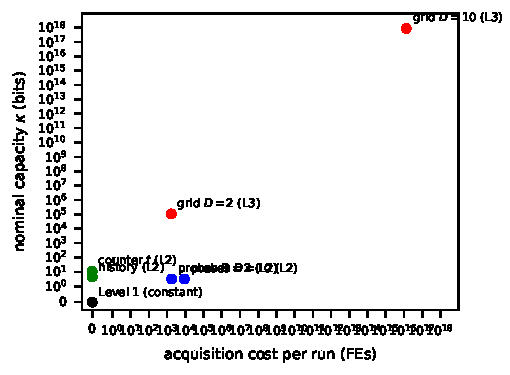
\includegraphics[width=0.92\columnwidth]{fig_info.pdf}
\caption{Nominal capacity versus acquisition cost of the information states in Table~\ref{tab:levels}. Level~3 is separated from the other levels by many orders of magnitude on both axes, while Level~2 states are cheap or cost a fraction of the budget.}
\label{fig:info}
\end{figure}

\subsection{Placement of known schemes}
Constant parameters are Level~1. Deterministic schedules (decaying $p$) condition on the counter, and feedback rules (success rates, stagnation counters, the 1/5 rule) condition on a bounded history summary; both are Level~2 with zero acquisition cost. Probe-based and learned feature policies are Level~2 with positive cost. These correspond to the deterministic and adaptive classes of Eiben et al.~\cite{eiben1999}. Self-adaptive schemes, population-level information and surrogate models are not placed.

\subsection{Level 3 as an engine instance}
A table of $f$ changes the global proposal and not only $p$: the natural proposal is a point mass at the table minimum, used once, after which the search refines locally with $p=0$. We therefore implement Level~3 in three forms: (a)~\emph{table-argmin}, which stops at the grid minimum; (b)~\emph{full grid + refinement} ($n=41$ at $D=2$), which uses the remaining FEs for hill climbing; and (c)~\emph{budget-matched grid + refinement}, with $n=\lfloor (B/2)^{1/D}\rfloor$ cell centres per axis (31 at $D=2$, 2 at $D=10$), so the grid uses about half the budget. For a deterministic and freely evaluable objective, the Bellman recursion on the grid reduces to taking the minimum, so no value iteration is used.

\subsection{What the framework does and does not predict}
The taxonomy is descriptive. It does not predict which policy performs best, because the value of information depends on the landscape. What it provides is an accounting identity. For a policy with acquisition cost, let a \emph{free variant} be the same policy with its acquisition evaluations not charged, and let the \emph{baseline} be a constant policy. Define, from median best fitness,
\begin{align}
V&=\frac{\mathrm{med}(\text{free})}{\mathrm{med}(\text{baseline})}, &
P&=\frac{\mathrm{med}(\text{charged})}{\mathrm{med}(\text{free})},\\
VP&=\frac{\mathrm{med}(\text{charged})}{\mathrm{med}(\text{baseline})}. & &
\end{align}
Information is \emph{relevant} when $V<1$ (it helps when free), \emph{affordable} when $P$ is small, and worth acquiring only when $VP<1$. Ratios of medians are unstable for bimodal outcomes and are descriptive only.

\section{Algorithms}
\subsection{Engine}
Algorithm~\ref{alg:search} is the single engine for Levels~1 and~2. The budget is strict: an iteration starts only if its full cost, including acquisition evaluations, fits into the remaining budget, so no run exceeds $B$ FEs.

\begin{algorithm}[t]
\caption{BJS Engine with Policy $\pi$ and Strict Budget}
\label{alg:search}
\begin{algorithmic}[1]
\REQUIRE Objective $f$, dimension $D$, budget $B$, policy $\pi$ with per-iteration cost $a$
\ENSURE Best fitness $f_x$
\STATE $x \leftarrow \mathcal{U}[l,u]^D$; $f_x \leftarrow f(x)$
\WHILE{FEs used $+\,(1{+}a) \le B$}
  \STATE $z \leftarrow \textsc{Acquire}(f,x,f_x,\text{history})$ \COMMENT{costs $a$ FEs}
  \STATE $(p,\sigma) \leftarrow \pi(z)$
  \IF{$\mathcal{U}[0,1] < p$}
    \STATE $x' \sim q(\cdot\mid z)$ \COMMENT{global jump, uniform for Levels 1--2}
  \ELSE
    \STATE $x' \leftarrow \operatorname{clip}\!\left(x + \mathcal{N}(0,\sigma^2 I),\ l,\ u\right)$
  \ENDIF
  \STATE $f' \leftarrow f(x')$
  \IF{$f' < f_x$}
    \STATE $x \leftarrow x'$; $f_x \leftarrow f'$
  \ENDIF
\ENDWHILE
\RETURN $f_x$
\end{algorithmic}
\end{algorithm}

\subsection{Policies}
\textbf{Constants (Level 1).} $p\in\{0,0.01,0.05,0.1,0.2,0.3,0.4,0.5,1\}$ with $\sigma=0.1$. For $p=0$, $\sigma\in\{0.003,0.01,0.03,0.3,1\}$ are added, and for $p=0.2$, $\sigma\in\{0.03,0.3\}$. The best fixed-$\sigma$ hill climber of each cell, $\sigma^\star$, is chosen in-sample, which favours it.

\textbf{ML-BJS (Level 2, probe-based).} The feature $\psi(x)$ is the fraction of $k=8$ Gaussian probes (standard deviation $0.1$) that improve on $f(x)$, so $\psi$ takes nine values and $\pi=\phi\circ\psi$ is a nine-entry table. The table is the prediction of a random forest (30 trees, \texttt{random\_state}$=0$, other scikit-learn defaults) trained on 300 uniformly random points of each of the unshifted Sphere (target $0.05$) and Rastrigin (target $0.8$) functions, separately for each $D$. The learned tables are $[0.70,0.59,0.42,0.40,0.42,0.39,0.49,0.40,0.80]$ ($D=2$) and $[0.58,0.46,0.39,0.41,0.40,0.44,0.43,0.59,0.80]$ ($D=10$), indexed by $\psi=0,\frac18,\dots,1$. Probes are charged. Training used $600\times9=5400$ evaluations, which are not charged; this is $2.7B$ at $D=2$ and $0.54B$ at $D=10$.

\textbf{ML-BJS variants.} \emph{Free-probe}: probes not charged (not budget-fair; isolates the cost). \emph{Reuse}: an improving probe is accepted as a move, so probes are not wasted. \emph{Probe/4}: probes only every fourth iteration. \emph{Train 1--4}: four further training replicates with new samples and forest seeds. \emph{Disjoint}: trained on Zakharov (target $0.05$) and Levy (target $0.8$)~\cite{jamil2013}, which are not test functions.

\textbf{History-BJS (Level 2, zero cost).} $p_t=0.05+0.5(1-a_t)$, where $a_t$ is the acceptance rate over the last 20 iterations ($p=0.2$ initially); a second variant uses $p_t=0.02+0.2(1-a_t)$. The forms were fixed before the experiments and not tuned.

\textbf{Decay-$p$ (Level 2, counter).} $p_t=0.5\,(1-n_t/B)$, where $n_t$ is the number of FEs used.

\textbf{1/5 rule (Level 2, zero cost).} A (1+1) strategy with $p=0$ in which $\sigma$ is multiplied by $1.5$ after a success and $1.5^{-1/4}$ after a failure, starting from $0.1$~\cite{rechenberg1973,schumer1968}. A joint variant applies the same rule to the local steps of BJS with $p=0.2$.

\textbf{Level 3.} The three forms of Section~\ref{sec:levels}.

\section{Experimental Setup}
\subsection{Benchmarks and instances}
Five functions on $[-5.12,5.12]^D$ with global minimum $0$ are used: Sphere, Rastrigin~\cite{torn1989}, Ackley~\cite{ackley1987} (constants $20$, $0.2$, $2\pi$), Griewank~\cite{griewank1981} and Rosenbrock~\cite{rosenbrock1960}. Each instance applies a random shift $g(x)=f(x-s)$ with $s\sim\mathcal{U}(-2,2)^D$, so the optimum is neither at the origin nor on a grid point. No rotation is applied. Because the local step is isotropic and the global jump is uniform, BJS is invariant to rotations of the landscape about the optimum, up to clipping at the domain boundary, so separability does not favour it. The dimensions are $D\in\{2,10\}$, with budget $B=1000D$ FEs; a larger-budget check uses $5B$ at $D=2$ and $3B$ at $D=10$ for five methods.

\subsection{Protocol and randomness}
Each method is run once on each of 30 instances, with the same 30 shifts for all methods. Each run draws from its own stream \texttt{default\_rng([seed, $D$, function index, method id])}, so runs are independent and reproducible. The result is the best fitness found. Values below $10^{-12}$ are at the floor of double precision and are treated as $10^{-12}$ in tests and shown as $<10^{-12}$. Medians and interquartile ranges (IQR) are reported. Success is defined as a final fitness of at most $10^{-2}$.

\subsection{Statistics}
Tests are paired by instance. Hypotheses were declared in two rounds. Round~1 (before the first experiments): H1, ML-BJS vs.\ $p=0.2$; H2, ML-BJS vs.\ its free-probe variant; H3, History-BJS vs.\ $p=0.2$; H4, the 1/5 rule vs.\ $p=0.2$. Round~2 (declared in the script header after seeing round-1 results and before running round~2): H5, the 1/5 rule vs.\ the best fixed-$\sigma$ hill climber; H6, free-probe ML-BJS vs.\ $p=0.2$; H7, probe-reuse vs.\ charged ML-BJS; H8, Decay-$p$ vs.\ $p=0.2$. Each is tested in the ten (dimension, function) cells with a two-sided Wilcoxon signed-rank test~\cite{wilcoxon1945}; zero differences are dropped, and an all-zero difference gives $p=1$. The 80 $p$-values are adjusted jointly by the Holm procedure~\cite{holm1979}. There is no external timestamp for the declarations, which should be read as declarations in the supplied scripts. Non-significance is not read as equivalence. Equivalence is assessed with two one-sided tests (TOST)~\cite{schuirmann1987} on the paired $\log_{10}$ ratio with a margin of a factor of two: E1, History-BJS vs.\ $p=0.2$; E2, free-probe ML-BJS vs.\ $p=0.4$ (Holm over 20 tests). The effect measure is the median paired $\log_{10}$ ratio (first over second; positive means the first method is worse). All other comparisons are descriptive ratios of medians. Level~3 is deterministic given the instance, so it is not tested.

\section{Results and Discussion}
\subsection{Overview}
Tables~\ref{tab:resD2} and~\ref{tab:resD10} give medians and IQRs of the budget-fair methods, Table~\ref{tab:l3} the Level~3 variants, Table~\ref{tab:tests} the 80 pre-declared tests, and Table~\ref{tab:value} the accounting quantities of Section~\ref{sec:levels} and the equivalence tests. Appendix tables report the variants, the realised-information diagnostics, the larger-budget check and the success counts. All runs respected the budget. Of the 80 tests, 30 were significant after correction.

\begin{table*}[t]
\centering
\caption{Median and IQR of Best Fitness, $D=2$, $B=2000$ FEs, 30 Shifted Instances}
\label{tab:resD2}
\scriptsize
\setlength{\tabcolsep}{1.5pt}
\begin{tabular}{@{}lccccccc@{}}
\toprule
 & $p{=}0$ & $p{=}0.2$ & $p{=}1$ & ML-BJS & Hist-BJS & Decay-$p$ & 1/5-rule\\
\midrule
Sphere & $5.95\mathrm{e}{-6}$ & $1.54\mathrm{e}{-5}$ & $0.0121$ & $5.21\mathrm{e}{-4}$ & $1.82\mathrm{e}{-5}$ & $8.46\mathrm{e}{-6}$ & $\mathbf{<\!10^{-12}}$ \\
\hspace{1em}IQR & $[3.1\mathrm{e}{-6},1.2\mathrm{e}{-5}]$ & $[6.6\mathrm{e}{-6},2.5\mathrm{e}{-5}]$ & $[5.2\mathrm{e}{-3},0.0175]$ & $[2.3\mathrm{e}{-4},8.9\mathrm{e}{-4}]$ & $[1.1\mathrm{e}{-5},3.6\mathrm{e}{-5}]$ & $[2.6\mathrm{e}{-6},1.8\mathrm{e}{-5}]$ & $[<\!10^{-12},<\!10^{-12}]$ \\
Rastrigin & $4.98$ & $1$ & $1.44$ & $2.06$ & $1$ & $\mathbf{0.998}$ & $12.9$ \\
\hspace{1em}IQR & $[3.98,8.96]$ & $[0.998,1.99]$ & $[1.13,1.75]$ & $[1.02,4.07]$ & $[0.996,1.01]$ & $[0.996,1.75]$ & $[5.97,16.9]$ \\
Ackley & $5.38$ & $0.0121$ & $0.564$ & $0.0891$ & $0.0157$ & $\mathbf{0.0104}$ & $10.2$ \\
\hspace{1em}IQR & $[3.57,6.56]$ & $[6.7\mathrm{e}{-3},0.0185]$ & $[0.303,0.996]$ & $[0.0419,2.58]$ & $[0.0108,0.0188]$ & $[7.3\mathrm{e}{-3},0.0163]$ & $[7.38,11.9]$ \\
Griewank & $\mathbf{6.15\mathrm{e}{-6}}$ & $7.40\mathrm{e}{-3}$ & $5.77\mathrm{e}{-3}$ & $7.44\mathrm{e}{-3}$ & $8.27\mathrm{e}{-4}$ & $7.40\mathrm{e}{-3}$ & $7.40\mathrm{e}{-3}$ \\
\hspace{1em}IQR & $[2.3\mathrm{e}{-6},0.125]$ & $[6.4\mathrm{e}{-6},7.4\mathrm{e}{-3}]$ & $[4.0\mathrm{e}{-3},7.8\mathrm{e}{-3}]$ & $[2.1\mathrm{e}{-3},7.6\mathrm{e}{-3}]$ & $[8.0\mathrm{e}{-6},7.4\mathrm{e}{-3}]$ & $[7.3\mathrm{e}{-6},7.4\mathrm{e}{-3}]$ & $[<\!10^{-12},7.4\mathrm{e}{-3}]$ \\
Rosenbrock & $\mathbf{7.31\mathrm{e}{-5}}$ & $1.90\mathrm{e}{-4}$ & $0.108$ & $0.258$ & $6.41\mathrm{e}{-4}$ & $1.76\mathrm{e}{-4}$ & $5.18\mathrm{e}{-3}$ \\
\hspace{1em}IQR & $[3.4\mathrm{e}{-5},2.0\mathrm{e}{-4}]$ & $[5.9\mathrm{e}{-5},5.6\mathrm{e}{-4}]$ & $[0.0345,0.221]$ & $[0.0406,0.519]$ & $[1.7\mathrm{e}{-4},1.4\mathrm{e}{-3}]$ & $[8.7\mathrm{e}{-5},3.4\mathrm{e}{-4}]$ & $[2.8\mathrm{e}{-3},0.0344]$ \\
\bottomrule
\end{tabular}

\smallskip
\footnotesize Bold: lowest median in the row (descriptive, no test). All columns are budget-fair ($\sigma=0.1$ except the 1/5-rule). Griewank outcomes are bimodal, so its medians are fragile.
\end{table*}

\begin{table*}[t]
\centering
\caption{Median and IQR of Best Fitness, $D=10$, $B=10{,}000$ FEs, 30 Shifted Instances}
\label{tab:resD10}
\scriptsize
\setlength{\tabcolsep}{1.5pt}
\begin{tabular}{@{}lccccccc@{}}
\toprule
 & $p{=}0$ & $p{=}0.2$ & $p{=}1$ & ML-BJS & Hist-BJS & Decay-$p$ & 1/5-rule\\
\midrule
Sphere & $9.42\mathrm{e}{-3}$ & $8.29\mathrm{e}{-3}$ & $12.4$ & $0.0264$ & $0.0117$ & $9.09\mathrm{e}{-3}$ & $\mathbf{<\!10^{-12}}$ \\
\hspace{1em}IQR & $[7.8\mathrm{e}{-3},0.011]$ & $[6.8\mathrm{e}{-3},9.7\mathrm{e}{-3}]$ & $[11.1,13.8]$ & $[0.0232,0.0335]$ & $[9.9\mathrm{e}{-3},0.0137]$ & $[7.6\mathrm{e}{-3},0.0107]$ & $[<\!10^{-12},<\!10^{-12}]$ \\
Rastrigin & $\mathbf{36.7}$ & $51.5$ & $70.4$ & $62.8$ & $52.1$ & $52.9$ & $93.5$ \\
\hspace{1em}IQR & $[29.8,44.7]$ & $[39.9,61.2]$ & $[66.7,74.6]$ & $[52.8,75.4]$ & $[39.5,60.3]$ & $[38.6,62.8]$ & $[69.4,128]$ \\
Ackley & $5.93$ & $\mathbf{4.83}$ & $5.64$ & $5.63$ & $4.89$ & $5.19$ & $8.94$ \\
\hspace{1em}IQR & $[4.94,6.24]$ & $[4.27,5.5]$ & $[5.43,5.85]$ & $[4.95,6.26]$ & $[3.98,5.17]$ & $[3.97,5.52]$ & $[4.33,9.9]$ \\
Griewank & $\mathbf{1.50\mathrm{e}{-3}}$ & $0.0333$ & $0.612$ & $0.129$ & $0.0285$ & $0.216$ & $0.143$ \\
\hspace{1em}IQR & $[1.1\mathrm{e}{-3},0.335]$ & $[0.0107,0.253]$ & $[0.523,0.678]$ & $[0.0147,0.366]$ & $[0.0167,0.223]$ & $[0.0242,0.367]$ & $[0.0111,0.475]$ \\
Rosenbrock & $8.37$ & $9.12$ & $2.53\mathrm{e}{3}$ & $11.9$ & $9.12$ & $8.45$ & $\mathbf{1.23}$ \\
\hspace{1em}IQR & $[7.51,9.85]$ & $[8.42,10.5]$ & $[2.0\mathrm{e}{3},3.8\mathrm{e}{3}]$ & $[10.8,89.7]$ & $[7.99,10.4]$ & $[7.21,10.1]$ & $[0.894,3.72]$ \\
\bottomrule
\end{tabular}

\smallskip
\footnotesize Notation as in Table~\ref{tab:resD2}. At $D=10$ the multimodal cells are near random-search level for all methods (no run reaches the success threshold, Table~\ref{tab:success}).
\end{table*}

\begin{figure*}[t]
\centering
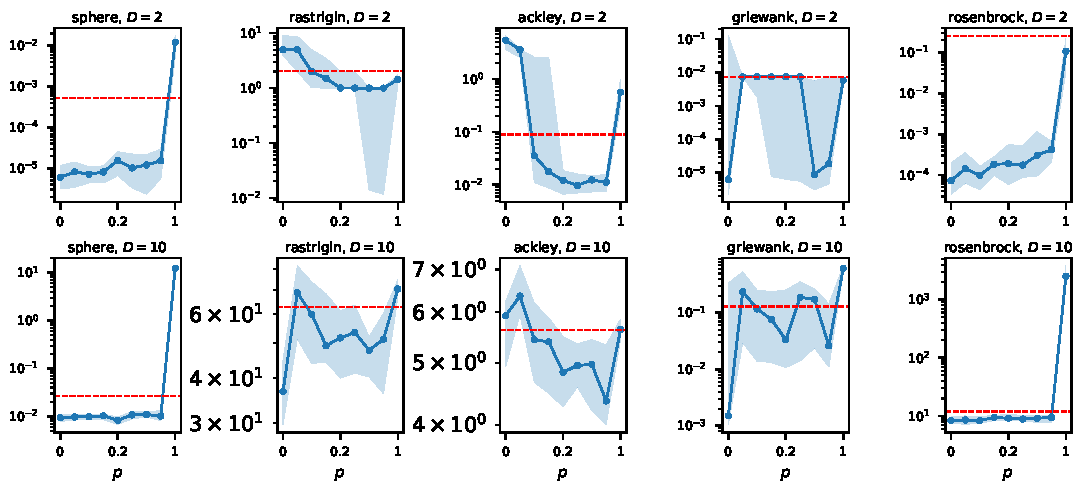
\includegraphics[width=0.9\textwidth]{fig_sweep2.pdf}
\caption{Constant-$p$ sweep (median and IQR band over 30 instances, log scale, $\sigma=0.1$). The dashed line is the median of ML-BJS. The horizontal axis shows $p\in\{0,0.01,0.05,0.1,0.2,0.3,0.4,0.5,1\}$ with ticks at $0$, $0.2$ and $1$.}
\label{fig:sweep}
\end{figure*}

\subsection{Level 1: constants, and the step size}
The best constant depends on the problem (Fig.~\ref{fig:sweep}). Over the nine constants, $p^\star=0$ in five cells and takes the values $0.4$, $0.3$, $0.2$, $0.5$ and $0.05$ in one cell each (Table~\ref{tab:value}). Hill climbing ($p=0$) is better than $p=0.2$ in six cells and worse in four, but materially worse only at $D=2$ on Rastrigin ($5.0\times$) and Ackley ($4.4\times10^{2}$); at $D=10$ it is $1.14\times$ (Sphere) and $1.23\times$ (Ackley) worse. Pure random search is worse than $p=0.2$ in nine cells, by up to $1.5\times10^{3}$ (Sphere, $D=10$), and better only on the bimodal Griewank at $D=2$ ($0.78\times$). The in-sample gain from using $p^\star$ instead of $0.2$ is at most $1.41\times$ in six cells and about $2.6\times$ in two ($D=2$ Sphere and Rosenbrock); for Griewank the ratios ($1.2\times10^{3}$, $22$) reflect unstable bimodal medians. These gains are optimistic because $p^\star$ is chosen on the same data, and they bound only the benefit of per-problem \emph{constants}; a policy that changes $p$ within a run is not bounded by them.

For Rastrigin at $D=2$, hill climbing ended in the basin of its random start in $93\%$ of runs, against $13\%$ for $p=0.2$ (nearest lattice minimum of the shifted function), which agrees with the explanation that greedy acceptance with $\sigma=0.1$ cannot cross the barriers. At $D=10$ the same criterion gives $20\%$ and $3\%$, but we do not interpret it, since a start near a basin boundary in any of ten coordinates breaks the criterion.

\emph{The step size is a major confounder.} For $p=0.2$, $\sigma=0.03$ lowers the median relative to $\sigma=0.1$ by $25\times$ ($D=2$ Sphere), $10\times$ ($D=10$ Sphere) and $7\times$ ($D=2$ Rosenbrock) and raises it by $3.5\times$ (Griewank, $D=10$); $\sigma=0.3$ raises it by up to $11\times$ (Sphere, $D=10$) but lowers it by $6\times$ (Ackley, $D=10$). The best fixed-$\sigma$ hill climber has a lower median than $p=0.2$ with $\sigma=0.1$ in nine of ten cells (for example $0.008\times$ on Sphere at $D=2$ and $0.002\times$ at $D=10$) and is $2.2\times$ worse only on Ackley at $D=2$. The chosen $\sigma^\star$ is $0.01$ and $0.003$ on Sphere, $1.0$ and $0.1$ on Rastrigin, and $0.3$ on Ackley; on Rastrigin at $D=2$ a large Gaussian step ($\sigma^\star=1$, median $0.081$) is far better than uniform jumps with $p=0.2$ (median $\approx1$), so the uniform global proposal is not an efficient exploration mechanism. All conclusions about $p$ are therefore conditional on $\sigma=0.1$.

As a sanity check, the median squared distance to the optimum of the best of $N$ uniform samples in a domain of area $A$ is approximately $A(1-2^{-1/N})/\pi=1.16\times10^{-2}$ for $N=2000$ and $A=10.24^2$. The measured median for $p=1$ on $D=2$ Sphere is $1.21\times10^{-2}$ ($+4.8\%$); a bootstrap interval (5000 resamples, seed 0) of the measured median, $[7.0\times10^{-3},1.7\times10^{-2}]$, contains the analytical value.

\subsection{Level 2: the probe-based policy}
\textbf{It never produced a net gain.} ML-BJS was significantly worse than $p=0.2$ in three of ten cells (H1: Sphere at $D=2$ and $D=10$, Rosenbrock at $D=2$) and never significantly better; the other seven were unresolved (Table~\ref{tab:tests}). In the accounting of Table~\ref{tab:value}, the net ratio $VP$ is at least $1.005$ in all ten cells, so in no cell did charged probes beat the constant baseline.

\textbf{The cost is significant.} Charging the probes made ML-BJS significantly worse than its free-probe variant in seven of ten cells (H2), with $P$ between $1.11$ and $341$; the three unresolved cells are at $D=10$. The two variants differ only in the accounting of the probe evaluations, so the effect is attributable to the cost. With nine evaluations per iteration, the engine performs about $222$ iterations at $D=2$ and $1111$ at $D=10$, instead of $2000$ and $10{,}000$. At the larger budget the penalty does not vanish: $P\ge1.15$ in all cells (Table~\ref{tab:large}).

\textbf{Free information was also uninformative.} The free-probe variant was not significantly different from $p=0.2$ in nine of ten cells (H6; it was significantly worse on Sphere at $D=10$), and its value ratio $V$ is below one only in three cells (Rastrigin at both dimensions, $0.996$ and $0.86$, and the bimodal Griewank at $D=2$, $5.8\times10^{-3}$). Equivalence with the constant $p=0.4$ within a factor of two (E2) holds in three cells ($D=10$ Sphere, Rastrigin and Ackley) and is unresolved elsewhere.

\textbf{Why the feature carried so little.} We measured what the policy uses (Appendix, Table~\ref{tab:real}). On the training data, the feature $\psi$ has $2.6$ bits of entropy but only $0.027$ bits ($D=2$) and $0.018$ bits ($D=10$) of mutual information with the binary training label, so a regressor on it can only approximate the label mean ($0.425$); the learned table entries deviate from that mean by $0.11$ and $0.09$ on average. In the training data, $\psi=0$ is rare ($1.0\%$ and $1.8\%$), but along search trajectories it is the most frequent state ($47$--$83\%$ of iterations), and its table entry ($0.70$ at $D=2$, $0.58$ at $D=10$) is among the largest. The realised $p$ therefore has mean $0.51$--$0.63$ and standard deviation $0.05$--$0.13$ and not $\approx0.4$, and the realised entropy of the policy output is only $0.8$--$1.6$ bits, against a nominal $3.17$. This is a covariate shift between uniform training points and search states, and a tested explanation of the near-constant policy. The hand-assigned targets remain a limitation.

\textbf{Design choices matter.} Reusing improving probes as moves significantly improved on the charged policy in four cells (H7: Sphere and Rosenbrock at both dimensions) and was never worse, but its median was below that of $p=0.2$ in only three cells ($D=2$ Sphere, $D=2$ and $D=10$ Rosenbrock). Probing every fourth iteration lowered the median relative to charged ML-BJS in all ten cells, but it was not below $p=0.2$ in any (descriptive). Across five training replicates the cell medians differ by a factor of $1.0$--$2.7$, except Ackley at $D=2$ ($42\times$), so a single training run (as in earlier drafts) was not representative there. A policy trained on disjoint functions was not below $p=0.2$ in any cell. The probe count $k=8$ was not varied.

\textbf{Larger budget.} At $5B$ ($D=2$), the free-probe and history policies reached the central Rastrigin basin (medians $2.8\times10^{-3}$ and $1.3\times10^{-3}$, against $0.995$ for $p=0.2$). Both realise $p\approx0.5$--$0.6$, and we did not run constants at the larger budget, so this cannot be attributed to information.

\subsection{Level 2: zero-cost history and schedules}
The rejection-rate rule was not significantly different from $p=0.2$ in any cell (H3); equivalence within a factor of two holds in three cells ($D=10$ Sphere, Rastrigin, Ackley; E1) and is unresolved in the rest. The realised $p$ has mean $0.54$--$0.55$ and standard deviation $0.01$--$0.03$ (first-quarter versus last-quarter mean $0.53$ versus $0.55$ on Rastrigin at $D=2$), and the realised entropy is $0.23$--$0.85$ bits against a nominal $4.39$. The rule therefore acts almost like a constant $p\approx0.54$; its medians are within $0.97$--$1.53\times$ of those of $p=0.5$ in nine cells (the Griewank outlier at $D=2$ is $44\times$). Its design constants are arbitrary, and a lower-range variant gave medians within $0.58$--$1.21\times$ of $p=0.2$ in eight cells (Griewank: $3.3\times$ at $D=10$ and an unstable $\approx0\times$ at $D=2$). The decaying schedule was not significantly different from $p=0.2$ in any cell (H8), had the lowest median among the seven budget-fair columns of Tables~\ref{tab:resD2}--\ref{tab:resD10} in two cells (Rastrigin and Ackley at $D=2$), and is within $0.55$--$1.1\times$ of $p=0.2$ in nine cells (Griewank at $D=10$: $6.5\times$, unstable). In this suite, zero-cost information about $p$ gave no measurable benefit.

\subsection{Zero-cost information about the step size}
The 1/5 rule was significantly better than $p=0.2$ in three cells (Sphere at both dimensions and Rosenbrock at $D=10$) and significantly worse in five (Rastrigin and Ackley at both dimensions, and Rosenbrock at $D=2$; H4). It reaches the numerical floor on Sphere. Against the best fixed-$\sigma$ hill climber (H5, in-sample choice of $\sigma^\star$, which favours the climber), it is significantly better on Sphere at both dimensions and significantly worse in the same five multimodal cells; three cells are unresolved. Adapting $\sigma$ from the success history costs no evaluations and is the largest zero-cost effect observed, but the rule loses on multimodal problems because it cannot leave a basin. Combining it with $p=0.2$ gave a median at or near the floor on Sphere (both dimensions), Ackley ($D=2$) and Griewank ($D=2$), and the highest success counts on Ackley at $D=2$ ($26/30$ against $13/30$ for $p=0.2$), but it was $38\times$ worse than $p=0.2$ on Rosenbrock at $D=2$ and $4.9\times$ worse on Griewank at $D=10$. Because these policies control $\sigma$ and the others control $p$, the comparison mixes information with parameterisation.

\subsection{Level 3: tabulated information}
\begin{table}[t]
\centering
\caption{Median Best Fitness of Level 3 Variants and References}
\label{tab:l3}
\scriptsize
\setlength{\tabcolsep}{1.6pt}
\begin{tabular}{@{}clccccc@{}}
\toprule
$D$ & Function & Table-argmin & Full+ref. & Matched+ref. & $p{=}0$ & $p{=}0.2$\\
\midrule
2 & Sphere & $0.01$ & $5.16\mathrm{e}{-5}$ & $1.78\mathrm{e}{-5}$ & $5.95\mathrm{e}{-6}$ & $1.54\mathrm{e}{-5}$ \\
2 & Rastrigin & $2.41$ & $0.0279$ & $3.61\mathrm{e}{-3}$ & $4.98$ & $1$ \\
2 & Ackley & $0.595$ & $0.022$ & $0.0126$ & $5.38$ & $0.0121$ \\
2 & Griewank & $3.89\mathrm{e}{-3}$ & $1.45\mathrm{e}{-5}$ & $1.01\mathrm{e}{-5}$ & $6.15\mathrm{e}{-6}$ & $7.40\mathrm{e}{-3}$ \\
2 & Rosenbrock & $0.134$ & $4.16\mathrm{e}{-3}$ & $1.39\mathrm{e}{-4}$ & $7.31\mathrm{e}{-5}$ & $1.90\mathrm{e}{-4}$ \\
\midrule
10 & Sphere & --- & --- & $0.0103$ & $9.42\mathrm{e}{-3}$ & $8.29\mathrm{e}{-3}$ \\
10 & Rastrigin & --- & --- & $33.8$ & $36.7$ & $51.5$ \\
10 & Ackley & --- & --- & $5.44$ & $5.93$ & $4.83$ \\
10 & Griewank & --- & --- & $8.47\mathrm{e}{-3}$ & $1.50\mathrm{e}{-3}$ & $0.0333$ \\
10 & Rosenbrock & --- & --- & $8.05$ & $8.37$ & $9.12$ \\
\bottomrule
\end{tabular}

\smallskip
\footnotesize $D=2$: $n=41$ (1681 FEs) and matched $n=31$ (961 FEs); $D=10$: matched $n=2$ (1024 FEs), full grid infeasible. ``+ref.'' uses the remaining FEs for hill climbing from the table minimum.
\end{table}

With shifted optima the grid is accurate only to its resolution. The table-argmin ($D=2$, 1681 FEs, error bounded by the resolution $h=0.256$; for Sphere at most $D(h/2)^2\approx3.3\times10^{-2}$) is worse than $p=0.2$ on four of five functions (by $651\times$, $2.4\times$, $49\times$ and $709\times$ on Sphere, Rastrigin, Ackley and Rosenbrock) and better only on Griewank ($0.53\times$, unstable). Adding refinement with the remaining $319$ FEs gives medians $5.2\times10^{-5}$, $2.8\times10^{-2}$, $2.2\times10^{-2}$, $1.5\times10^{-5}$ and $4.2\times10^{-3}$, which is better than $p=0.2$ on Rastrigin ($0.028\times$) and Griewank ($0.002\times$) and worse on Sphere ($3.4\times$), Ackley ($1.8\times$) and Rosenbrock ($22\times$).

The budget-matched grid with refinement is better than $p=0.2$ in six of ten cells (at $D=2$: Rastrigin, with median $3.6\times10^{-3}$ against $1.0$, Griewank and Rosenbrock; at $D=10$: Rastrigin, Griewank and Rosenbrock) and worse in four by $1.04$--$1.25\times$ (Sphere and Ackley at both dimensions). On Rastrigin at $D=2$ it reaches the success threshold in $27/30$ runs, against at most $7/30$ for any other method. The information is worth its cost when the grid resolves the landscape: at $D=2$, $n=31$ resolves Rastrigin's lattice (spacing $1$) and hill climbing then refines. At $D=10$ the matched grid has two points per axis and carries almost no usable information: its medians are within $0.92$--$1.10\times$ of those of plain hill climbing in four cells (Sphere, Rastrigin, Ackley and Rosenbrock), and $5.7\times$ worse on Griewank, so its comparison with $p=0.2$ there mostly reflects the strength of hill climbing. The cost $n^D$ is $68{,}921$ FEs at $D=3$ and $1.3\times10^{16}$ at $D=10$. The earlier origin-centred configuration, in which the table-argmin was exact, was an alignment artifact.

\begin{table*}[t]
\centering
\caption{Pre-Declared Paired Tests: Median Paired $\log_{10}$ Ratio (Holm-Adjusted $p$ over 80 Tests)}
\label{tab:tests}
\scriptsize
\setlength{\tabcolsep}{2pt}
\begin{tabular}{@{}clcccccccc@{}}
\toprule
$D$ & Function & H1 & H2 & H3 & H4 & H5 & H6 & H7 & H8\\
 & & ML/0.2 & ML/free & Hist/0.2 & 1/5/0.2 & 1/5/best-$\sigma$ & free/0.2 & reuse/ML & decay/0.2\\
\midrule
2 & Sphere & +1.5 ($<$.001)$^\dagger$ & +1.5 ($<$.001)$^\dagger$ & +0.2 (1) & -7.2 ($<$.001)$^\dagger$ & -5.1 ($<$.001)$^\dagger$ & +0.1 (1) & -2.0 ($<$.001)$^\dagger$ & -0.1 (1) \\
2 & Rastrigin & +0.3 (.409) & +0.6 ($<$.001)$^\dagger$ & -0.0 (1) & +0.9 ($<$.001)$^\dagger$ & +2.2 ($<$.001)$^\dagger$ & -0.3 (.105) & -0.0 (1) & -0.0 (1) \\
2 & Ackley & +0.9 (.078) & +0.7 ($<$.001)$^\dagger$ & +0.1 (1) & +2.9 ($<$.001)$^\dagger$ & +2.5 ($<$.001)$^\dagger$ & +0.2 (1) & -0.0 (1) & -0.1 (1) \\
2 & Griewank & +0.0 (.409) & +1.9 (.008)$^\dagger$ & -0.0 (1) & -0.0 (1) & -1.3 (1) & +0.0 (1) & -0.0 (1) & -0.0 (1) \\
2 & Rosenbrock & +2.9 ($<$.001)$^\dagger$ & +2.7 ($<$.001)$^\dagger$ & +0.3 (1) & +1.6 ($<$.001)$^\dagger$ & +2.2 (.002)$^\dagger$ & +0.4 (1) & -3.0 ($<$.001)$^\dagger$ & -0.2 (1) \\
\midrule
10 & Sphere & +0.5 ($<$.001)$^\dagger$ & +0.3 ($<$.001)$^\dagger$ & +0.1 (.067) & -9.9 ($<$.001)$^\dagger$ & -7.1 ($<$.001)$^\dagger$ & +0.1 ($<$.001)$^\dagger$ & -0.5 ($<$.001)$^\dagger$ & +0.0 (1) \\
10 & Rastrigin & +0.1 (.409) & +0.1 (.160) & -0.0 (1) & +0.3 ($<$.001)$^\dagger$ & +0.4 ($<$.001)$^\dagger$ & +0.0 (1) & -0.1 (1) & -0.0 (1) \\
10 & Ackley & +0.0 (.279) & +0.0 (1) & -0.0 (1) & +0.2 (.007)$^\dagger$ & +0.9 ($<$.001)$^\dagger$ & +0.0 (1) & +0.0 (1) & -0.0 (1) \\
10 & Griewank & +0.1 (1) & -0.0 (1) & +0.2 (1) & +0.2 (1) & +0.9 (1) & +0.1 (1) & -0.0 (1) & +0.3 (.140) \\
10 & Rosenbrock & +0.2 (.657) & +0.1 ($<$.001)$^\dagger$ & -0.0 (1) & -1.0 ($<$.001)$^\dagger$ & -0.5 (.463) & -0.0 (1) & -0.2 ($<$.001)$^\dagger$ & -0.1 (1) \\
\bottomrule
\end{tabular}

\smallskip
\footnotesize Positive: the first method is worse. $^\dagger$Holm-adjusted $p<0.05$. Pairs matched by instance; values clipped at $10^{-12}$.
\end{table*}

\begin{table*}[t]
\centering
\caption{Accounting of Information and Equivalence Tests (Descriptive Ratios of Medians; Holm $p$ for TOST over 20 Tests)}
\label{tab:value}
\scriptsize
\setlength{\tabcolsep}{3pt}
\begin{tabular}{@{}clccccccc@{}}
\toprule
$D$ & Function & $p^\star$ & $\frac{\mathrm{med}(p{=}0.2)}{\mathrm{med}(p^\star)}$ & $V$ & $P$ & $VP$ & E1: Hist $\equiv0.2$ & E2: free $\equiv0.4$\\
\midrule
2 & Sphere & 0 & 2.58 & 1.14 & 30 & 34 & 1 & 1 \\
2 & Rastrigin & 0.4 & 1.01 & 1.00 & 2.06 & 2.06 & 1 & 1 \\
2 & Ackley & 0.3 & 1.24 & 1.57 & 4.67 & 7.35 & 1 & 1 \\
2 & Griewank & 0 & $1.2\times10^{3}$ & $5.8\times10^{-3}$ & 175 & 1.01 & 1 & 1 \\
2 & Rosenbrock & 0 & 2.60 & 3.98 & 341 & $1.4\times10^{3}$ & 1 & 1 \\
\midrule
10 & Sphere & 0.2 & 1.00 & 1.47 & 2.17 & 3.18 & $<$.001$^\ddagger$ & $<$.001$^\ddagger$ \\
10 & Rastrigin & 0 & 1.41 & 0.86 & 1.41 & 1.22 & $<$.001$^\ddagger$ & $<$.001$^\ddagger$ \\
10 & Ackley & 0.5 & 1.11 & 1.04 & 1.11 & 1.16 & $<$.001$^\ddagger$ & $<$.001$^\ddagger$ \\
10 & Griewank & 0 & 22 & 3.23 & 1.21 & 3.89 & 1 & 1 \\
10 & Rosenbrock & 0.05 & 1.10 & 1.01 & 1.30 & 1.30 & .201 & .184 \\
\bottomrule
\end{tabular}

\smallskip
\footnotesize $V$: free-probe ML-BJS over $p=0.2$; $P$: charged over free-probe; $VP$: charged ML-BJS over $p=0.2$. $p^\star$: best of nine constants (in-sample). $^\ddagger$Equivalent within a factor of two (Holm $p<0.05$). Griewank ratios are unstable.
\end{table*}

\subsection{Synthesis}
Performance does not follow nominal capacity. The experiments separate four kinds of information. (i)~Probe information about $p$ was costly ($P$ up to $341$), barely informative as trained ($0.02$--$0.03$ bits), and never produced a net gain. (ii)~Zero-cost history and counter information about $p$ yielded policies that were close to constants ($R\le0.85$ bits). (iii)~Zero-cost history information about $\sigma$ was very valuable on smooth problems and harmful on multimodal ones. (iv)~Table information had high value when the grid resolved the landscape ($D=2$) and negligible value when it could not ($D=10$), at a cost exponential in $D$. What the taxonomy contributes is the accounting that separates these cases: capacity alone would rank the counter above the probe, and neither ranking matches the results. We do not claim that the hierarchy predicts the outcomes.

\subsection{Limitations}\label{sec:limits}
The experiments cover single-solution BJS-type variants. Population methods, annealing, DE and CMA-ES are not compared, so no claim is made about heuristic search in general. Dimensions are at most $10$; at $D=10$ the multimodal cells are near random-search level for every method and say little about control policies. A single budget family ($1000D$, with a larger-budget check for five methods) is used. Benchmarks are five classical functions with shifts in $[-2,2]$, without noise or constraints; rotation is argued to be irrelevant for BJS but was not run. The sweep has nine values of $p$ and the best constant and $\sigma^\star$ are chosen in-sample. The probe count $k=8$ was not varied. ML-BJS uses hand-assigned targets and uniformly random training points; its training cost is not charged, and since no tested variant beat $p=0.2$, no amortisation break-even exists. The reuse and probe-schedule variants were not tuned. Medians are unstable for the bimodal Griewank outcomes, and ratios of medians are descriptive. With 30 instances the tests have limited power, and non-significant results mean that differences were unresolved. The hypothesis declarations lack an external timestamp. Realised information is estimated by plug-in entropies of binned outputs. Finally, $\kappa$ is a nominal upper bound.

\section{Conclusion}
This paper classified single-solution BJS search by how the information state of its control policy scales with dimension, and measured nominal capacity, acquisition cost and realised information. Under a strict budget on shifted benchmarks, a learned probe-based policy for $p$ never produced a net gain, because its probes were costly and its feature carried almost no information at the states where it was used; zero-cost history and schedule policies for $p$ behaved like constants; zero-cost information about the step size was the most valuable and the most landscape-dependent; and table information was valuable only where the grid resolved the landscape. The conclusions are conditional on $\sigma=0.1$ and on the single-solution scope. Future work will add population-based and annealing baselines, higher dimensions and rotated benchmarks, varied probe counts and probe-reuse designs trained on search outcomes with disjoint training and test functions, and joint control of $p$ and $\sigma$ with equal information budgets.

\section*{Code and Data Availability}
Round~1 experiments (\texttt{experiments.py}), round~2 experiments (\texttt{experiments2.py}), the realised-information diagnostics (\texttt{logging\_exp.py}), the analysis (\texttt{analysis2.py}) and the figure script (\texttt{fig\_info.py}) reproduce all results; raw outputs are in \texttt{raw\_D2.csv}, \texttt{raw\_D10.csv}, \texttt{raw2\_D2.csv}, \texttt{raw2\_D10.csv} and \texttt{logging\_out.json}. The environment was Python 3.12.3, NumPy 2.4.4, SciPy 1.17.1, scikit-learn 1.8.0 and Matplotlib 3.10.8. All files will be deposited in a public repository at [REPOSITORY URL TO BE ADDED].

\appendices
\section{Additional Results}
\begin{table*}[t]
\centering
\caption{Median Best Fitness of Level 2 Variants ($\sigma=0.1$ Unless Stated; Budget-Fair Except Free-Probe)}
\label{tab:var}
\scriptsize
\setlength{\tabcolsep}{2pt}
\begin{tabular}{@{}clcccccccc@{}}
\toprule
$D$ & Function & ML free-probe & ML reuse & ML probe/4 & ML train 0--4 (min--max) & ML disjoint & Hist low & 1/5$\sigma$+0.2 & best-$\sigma$ HC\\
\midrule
2 & Sphere & $1.75\mathrm{e}{-5}$ & $7.48\mathrm{e}{-6}$ & $8.51\mathrm{e}{-5}$ & $2.6\mathrm{e}{-4}$--$5.2\mathrm{e}{-4}$ & $1.79\mathrm{e}{-4}$ & $8.91\mathrm{e}{-6}$ & $<\!10^{-12}$ & $1.20\mathrm{e}{-7}$ ($\sigma{=}0.01$) \\
2 & Rastrigin & $0.998$ & $1.99$ & $1.1$ & $1.1$--$2.1$ & $2.01$ & $0.997$ & $0.995$ & $0.0815$ ($\sigma{=}1$) \\
2 & Ackley & $0.0191$ & $1.16$ & $0.0358$ & $0.062$--$2.6$ & $0.128$ & $0.0127$ & $<\!10^{-12}$ & $0.0262$ ($\sigma{=}0.3$) \\
2 & Griewank & $4.26\mathrm{e}{-5}$ & $7.40\mathrm{e}{-3}$ & $7.42\mathrm{e}{-3}$ & $7.4\mathrm{e}{-3}$--$7.5\mathrm{e}{-3}$ & $7.44\mathrm{e}{-3}$ & $1.95\mathrm{e}{-5}$ & $<\!10^{-12}$ & $6.15\mathrm{e}{-6}$ ($\sigma{=}0.1$) \\
2 & Rosenbrock & $7.55\mathrm{e}{-4}$ & $1.78\mathrm{e}{-4}$ & $0.0135$ & $0.13$--$0.29$ & $0.119$ & $1.53\mathrm{e}{-4}$ & $7.27\mathrm{e}{-3}$ & $2.42\mathrm{e}{-5}$ ($\sigma{=}0.03$) \\
\midrule
10 & Sphere & $0.0122$ & $9.12\mathrm{e}{-3}$ & $0.0187$ & $0.02$--$0.036$ & $0.0258$ & $0.01$ & $<\!10^{-12}$ & $1.30\mathrm{e}{-5}$ ($\sigma{=}0.003$) \\
10 & Rastrigin & $44.4$ & $54.2$ & $56.4$ & $49$--$63$ & $55.9$ & $55.7$ & $53.2$ & $36.7$ ($\sigma{=}0.1$) \\
10 & Ackley & $5.05$ & $5.79$ & $5.25$ & $5.5$--$5.9$ & $5.87$ & $5.24$ & $4.78$ & $0.769$ ($\sigma{=}0.3$) \\
10 & Griewank & $0.107$ & $0.17$ & $0.0747$ & $0.051$--$0.14$ & $0.101$ & $0.111$ & $0.162$ & $1.50\mathrm{e}{-3}$ ($\sigma{=}0.1$) \\
10 & Rosenbrock & $9.16$ & $8.89$ & $10.4$ & $12$--$13$ & $12.5$ & $8.16$ & $1.96$ & $3.31$ ($\sigma{=}0.01$) \\
\bottomrule
\end{tabular}
\end{table*}

\begin{table*}[t]
\centering
\caption{Realised Policy Behaviour in Runs: ML-BJS (Charged) and History-BJS}
\label{tab:real}
\scriptsize
\setlength{\tabcolsep}{3.5pt}
\begin{tabular}{@{}clcccccccc@{}}
\toprule
 & & \multicolumn{5}{c}{ML-BJS} & \multicolumn{3}{c}{History-BJS}\\
\cmidrule(lr){3-7}\cmidrule(lr){8-10}
$D$ & Function & mean $p$ & sd $p$ & frac.\ $\psi{=}0$ & $H(\psi)$ & $H(p)$ & mean $p$ & sd $p$ & $H(p)$\\
\midrule
2 & Sphere & 0.58 & 0.13 & 0.47 & 2.31 & 1.59 & 0.54 & 0.03 & 0.57 \\
2 & Rastrigin & 0.63 & 0.11 & 0.64 & 1.62 & 1.33 & 0.54 & 0.03 & 0.58 \\
2 & Ackley & 0.61 & 0.12 & 0.56 & 1.96 & 1.51 & 0.54 & 0.03 & 0.66 \\
2 & Griewank & 0.62 & 0.12 & 0.63 & 1.85 & 1.39 & 0.54 & 0.03 & 0.59 \\
2 & Rosenbrock & 0.61 & 0.12 & 0.54 & 1.97 & 1.52 & 0.54 & 0.03 & 0.85 \\
\midrule
10 & Sphere & 0.52 & 0.08 & 0.60 & 1.97 & 1.36 & 0.54 & 0.03 & 0.45 \\
10 & Rastrigin & 0.56 & 0.05 & 0.83 & 0.89 & 0.80 & 0.55 & 0.01 & 0.23 \\
10 & Ackley & 0.55 & 0.06 & 0.77 & 1.20 & 1.00 & 0.55 & 0.02 & 0.33 \\
10 & Griewank & 0.51 & 0.08 & 0.56 & 1.98 & 1.43 & 0.55 & 0.02 & 0.45 \\
10 & Rosenbrock & 0.51 & 0.08 & 0.52 & 2.13 & 1.47 & 0.54 & 0.03 & 0.52 \\
\bottomrule
\end{tabular}

\smallskip
\footnotesize Pooled over 30 instances. $H(\psi)$: entropy in bits of visited probe fractions (nominal maximum $3.17$). $H(p)$: entropy in bits of the realised $p$ binned to $0.05$ (nominal maximum $3.17$ for ML-BJS and $4.39$ for History-BJS).
\end{table*}

\begin{table*}[t]
\centering
\caption{Larger Budget ($5B$ at $D=2$, $3B$ at $D=10$), Median Best Fitness (Descriptive, Not Tested)}
\label{tab:large}
\scriptsize
\setlength{\tabcolsep}{3pt}
\begin{tabular}{@{}clccccccc@{}}
\toprule
$D$ & Function & $p{=}0.2$ & ML-BJS & ML free-probe & Hist-BJS & 1/5-rule & $P$ (large) & $P$ (base)\\
\midrule
2 & Sphere & $1.40\mathrm{e}{-6}$ & $4.23\mathrm{e}{-5}$ & $4.54\mathrm{e}{-6}$ & $3.74\mathrm{e}{-6}$ & $<\!10^{-12}$ & 9.33 & 30 \\
2 & Rastrigin & $0.995$ & $1.01$ & $2.79\mathrm{e}{-3}$ & $1.25\mathrm{e}{-3}$ & $14.4$ & 363 & 2.06 \\
2 & Ackley & $5.26\mathrm{e}{-3}$ & $0.0317$ & $5.78\mathrm{e}{-3}$ & $6.31\mathrm{e}{-3}$ & $8.39$ & 5.49 & 4.67 \\
2 & Griewank & $1.24\mathrm{e}{-6}$ & $7.40\mathrm{e}{-3}$ & $1.44\mathrm{e}{-6}$ & $1.44\mathrm{e}{-6}$ & $7.40\mathrm{e}{-3}$ & $5.2\times10^{3}$ & 175 \\
2 & Rosenbrock & $1.78\mathrm{e}{-5}$ & $2.55\mathrm{e}{-3}$ & $5.39\mathrm{e}{-5}$ & $4.94\mathrm{e}{-5}$ & $1.89\mathrm{e}{-7}$ & 47 & 341 \\
\midrule
10 & Sphere & $7.27\mathrm{e}{-3}$ & $0.0164$ & $8.52\mathrm{e}{-3}$ & $8.01\mathrm{e}{-3}$ & $<\!10^{-12}$ & 1.92 & 2.17 \\
10 & Rastrigin & $47.4$ & $55.2$ & $46.1$ & $42.5$ & $94.5$ & 1.20 & 1.41 \\
10 & Ackley & $4.52$ & $5.14$ & $4.47$ & $4.28$ & $8.37$ & 1.15 & 1.11 \\
10 & Griewank & $0.135$ & $0.087$ & $0.0132$ & $0.0377$ & $0.115$ & 6.61 & 1.21 \\
10 & Rosenbrock & $7.93$ & $10.4$ & $8.67$ & $8.24$ & $0.0729$ & 1.20 & 1.30 \\
\bottomrule
\end{tabular}
\end{table*}

\begin{table*}[t]
\centering
\caption{Success Counts out of 30 (Final Fitness $\le10^{-2}$); Bold: Highest in Row}
\label{tab:success}
\scriptsize
\setlength{\tabcolsep}{2.5pt}
\begin{tabular}{@{}clcccccccccc@{}}
\toprule
$D$ & Function & $p{=}0$ & $p{=}0.2$ & $p{=}1$ & ML & ML free & Hist & Decay & 1/5 & 1/5$\sigma$+0.2 & L3 matched+ref.\\
\midrule
2 & Sphere & \textbf{30} & \textbf{30} & 12 & \textbf{30} & \textbf{30} & \textbf{30} & \textbf{30} & \textbf{30} & \textbf{30} & \textbf{30} \\
2 & Rastrigin & 0 & 3 & 0 & 0 & 6 & 7 & 5 & 1 & 4 & \textbf{27} \\
2 & Ackley & 1 & 13 & 0 & 1 & 5 & 5 & 14 & 1 & \textbf{26} & 9 \\
2 & Griewank & 18 & \textbf{30} & 29 & 29 & \textbf{30} & 29 & \textbf{30} & 29 & 29 & \textbf{30} \\
2 & Rosenbrock & \textbf{30} & 29 & 3 & 4 & 26 & 28 & 29 & 17 & 19 & \textbf{30} \\
\midrule
10 & Sphere & 19 & 23 & 0 & 1 & 9 & 8 & 19 & \textbf{30} & \textbf{30} & 12 \\
10 & Rastrigin & 0 & 0 & 0 & 0 & 0 & 0 & 0 & 0 & 0 & 0 \\
10 & Ackley & 0 & 0 & 0 & 0 & 0 & 0 & 0 & 0 & 0 & 0 \\
10 & Griewank & 16 & 7 & 0 & 2 & 2 & 4 & 6 & 8 & 6 & \textbf{27} \\
10 & Rosenbrock & 0 & 0 & 0 & 0 & 0 & 0 & 0 & 0 & 0 & 0 \\
\bottomrule
\end{tabular}
\end{table*}

\begin{thebibliography}{99}

\bibitem{sorensen2015}
K. S\"{o}rensen, ``Metaheuristics---the metaphor exposed,'' \emph{Int. Trans. Oper. Res.}, vol. 22, no. 1, pp. 3--18, 2015.

\bibitem{geem2001}
Z. W. Geem, J. H. Kim, and G. V. Loganathan, ``A new heuristic optimization algorithm: Harmony search,'' \emph{Simulation}, vol. 76, no. 2, pp. 60--68, 2001.

\bibitem{eiben1999}
A. E. Eiben, R. Hinterding, and Z. Michalewicz, ``Parameter control in evolutionary algorithms,'' \emph{IEEE Trans. Evol. Comput.}, vol. 3, no. 2, pp. 124--141, 1999.

\bibitem{karafotias2015}
G. Karafotias, M. Hoogendoorn, and A. E. Eiben, ``Parameter control in evolutionary algorithms: Trends and challenges,'' \emph{IEEE Trans. Evol. Comput.}, vol. 19, no. 2, pp. 167--187, 2015.

\bibitem{schumer1968}
M. A. Schumer and K. Steiglitz, ``Adaptive step size random search,'' \emph{IEEE Trans. Autom. Control}, vol. 13, no. 3, pp. 270--276, 1968.

\bibitem{rechenberg1973}
I. Rechenberg, \emph{Evolutionsstrategie: Optimierung technischer Systeme nach Prinzipien der biologischen Evolution}. Stuttgart, Germany: Frommann-Holzboog, 1973.

\bibitem{fialho2010}
\'{A}. Fialho, L. Da Costa, M. Schoenauer, and M. Sebag, ``Analyzing bandit-based adaptive operator selection mechanisms,'' \emph{Ann. Math. Artif. Intell.}, vol. 60, no. 1--2, pp. 25--64, 2010.

\bibitem{sharma2019}
M. Sharma, A. Komninos, M. L\'{o}pez-Ib\'{a}\~{n}ez, and D. Kazakov, ``Deep reinforcement learning based parameter control in differential evolution,'' in \emph{Proc. GECCO}, 2019, pp. 709--717.

\bibitem{burke2013}
E. K. Burke \emph{et al.}, ``Hyper-heuristics: A survey of the state of the art,'' \emph{J. Oper. Res. Soc.}, vol. 64, no. 12, pp. 1695--1724, 2013.

\bibitem{lourenco2003}
H. R. Louren\c{c}o, O. C. Martin, and T. St\"{u}tzle, ``Iterated local search,'' in \emph{Handbook of Metaheuristics}, F. Glover and G. Kochenberger, Eds. Boston, MA, USA: Kluwer, 2003, pp. 320--353.

\bibitem{zabinsky1992}
Z. B. Zabinsky and R. L. Smith, ``Pure adaptive search in global optimization,'' \emph{Math. Program.}, vol. 53, pp. 323--338, 1992.

\bibitem{yao1999}
X. Yao, Y. Liu, and G. Lin, ``Evolutionary programming made faster,'' \emph{IEEE Trans. Evol. Comput.}, vol. 3, no. 2, pp. 82--102, 1999.

\bibitem{doerr2017}
B. Doerr, H. P. Le, R. Makhmara, and T. D. Nguyen, ``Fast genetic algorithms,'' in \emph{Proc. GECCO}, 2017, pp. 777--784.

\bibitem{droste2006}
S. Droste, T. Jansen, and I. Wegener, ``Upper and lower bounds for randomized search heuristics in black-box optimization,'' \emph{Theory Comput. Syst.}, vol. 39, no. 4, pp. 525--544, 2006.

\bibitem{solis1981}
F. J. Solis and R. J.-B. Wets, ``Minimization by random search techniques,'' \emph{Math. Oper. Res.}, vol. 6, no. 1, pp. 19--30, 1981.

\bibitem{bergstra2012}
J. Bergstra and Y. Bengio, ``Random search for hyper-parameter optimization,'' \emph{J. Mach. Learn. Res.}, vol. 13, pp. 281--305, 2012.

\bibitem{shahriari2016}
B. Shahriari \emph{et al.}, ``Taking the human out of the loop: A review of Bayesian optimization,'' \emph{Proc. IEEE}, vol. 104, no. 1, pp. 148--175, 2016.

\bibitem{kirkpatrick1983}
S. Kirkpatrick, C. D. Gelatt, and M. P. Vecchi, ``Optimization by simulated annealing,'' \emph{Science}, vol. 220, no. 4598, pp. 671--680, 1983.

\bibitem{wolpert1997}
D. H. Wolpert and W. G. Macready, ``No free lunch theorems for optimization,'' \emph{IEEE Trans. Evol. Comput.}, vol. 1, no. 1, pp. 67--82, 1997.

\bibitem{torn1989}
A. T\"{o}rn and A. \v{Z}ilinskas, \emph{Global Optimization}, Lecture Notes in Computer Science, vol. 350. Berlin, Germany: Springer, 1989.

\bibitem{ackley1987}
D. H. Ackley, \emph{A Connectionist Machine for Genetic Hillclimbing}. Boston, MA, USA: Kluwer, 1987.

\bibitem{griewank1981}
A. O. Griewank, ``Generalized descent for global optimization,'' \emph{J. Optim. Theory Appl.}, vol. 34, no. 1, pp. 11--39, 1981.

\bibitem{rosenbrock1960}
H. H. Rosenbrock, ``An automatic method for finding the greatest or least value of a function,'' \emph{Comput. J.}, vol. 3, no. 3, pp. 175--184, 1960.

\bibitem{jamil2013}
M. Jamil and X.-S. Yang, ``A literature survey of benchmark functions for global optimisation problems,'' \emph{Int. J. Math. Model. Numer. Optim.}, vol. 4, no. 2, pp. 150--194, 2013.

\bibitem{wilcoxon1945}
F. Wilcoxon, ``Individual comparisons by ranking methods,'' \emph{Biometrics Bulletin}, vol. 1, no. 6, pp. 80--83, 1945.

\bibitem{holm1979}
S. Holm, ``A simple sequentially rejective multiple test procedure,'' \emph{Scand. J. Statist.}, vol. 6, no. 2, pp. 65--70, 1979.

\bibitem{schuirmann1987}
D. J. Schuirmann, ``A comparison of the two one-sided tests procedure and the power approach for assessing the equivalence of average bioavailability,'' \emph{J. Pharmacokinet. Biopharm.}, vol. 15, no. 6, pp. 657--680, 1987.

\end{thebibliography}

\end{document}
